\documentclass[12pt,a4paper]{article}
\usepackage{amsmath, amssymb}
\usepackage{geometry}
\usepackage{hyperref}
\usepackage{booktabs}
\usepackage{graphicx}
\usepackage{setspace}
\usepackage{float}
\usepackage{tikz}
\usetikzlibrary{automata, positioning, arrows}
\usepackage{xcolor}
\usepackage{listings}

\graphicspath{{assets/}}

\geometry{margin=1in}
\onehalfspacing

% ---------- Listings setup ----------
\lstdefinestyle{mypython}{
    language=Python,
    basicstyle=\ttfamily\small,
    keywordstyle=\color{blue},
    commentstyle=\color{gray},
    stringstyle=\color{teal},
    showstringspaces=false,
    numberstyle=\tiny,
    numbers=left,
    numbersep=8pt,
    frame=single,
    breaklines=true,
    tabsize=4
}
\lstset{style=mypython}
% ------------------------------------

\begin{document}

% Title Page
\begin{titlepage}
	\centering
	    
	\Huge
	\textbf{Jaypee Institute of Information Technology, Sector - 62, Noida } \\
	\vspace{0.5cm}
	\Large
	\textbf{B.Tech CSE III Semester}\\
	\vspace{1cm}
	\vspace*{\fill}
	    
	\includegraphics[scale=0.2]{jiit_logo}\\
	    
	\vspace{1.5cm}
	\Huge
	\textbf{Theory of Computation PBL Report}\\
	\Large
	    
	\textbf{Natural Language Processing using Automata}\\
	\vspace{1cm}
	
	\Large
	\textbf{Submitted to}\\
	Mr. Akshit Raj Patel
	\vspace{1cm}
	
	\textbf{Submitted by}
	\vspace{0.5cm}
	
	\begin{tabular}{lll}
		Harsh Sharma      & 2401030232 & B5 \\
		Karvy Singh       & 2401030234 & B5 \\
		Rudra Kumar Singh & 2401030237 & B5 \\
	\end{tabular}
	
	\vspace*{\fill}
	\normalsize
\end{titlepage}

%letter of transmittal 
\begin{center}
	\Large\textbf{Letter of Transmittal}
\end{center}
\vspace{1cm}

\noindent
\textbf{Mr. Akshit Raj Patel} \\
[0.5em]
Department of Computer Science \& IT\\
[0.5em]

\vspace{1cm}

\noindent
\textbf{Subject:} Submission of Project ``Natural Language Processing using Automata''

\vspace{1cm}

\noindent
Respected Sir,

\vspace{1em}

\noindent
We are pleased to submit our project titled \textit{``Natural Language Processing using Automata''} as part of our coursework for the Theory of Computation course. This report documents the design and implementation of a small natural language processing pipeline that uses concepts from deterministic finite automata (DFA) and context-free grammars (CFG) for tokenization and parsing of English sentences. 

\vspace{1em}

\noindent
We have endeavored to connect theoretical ideas from automata theory and formal languages to a practical Python implementation. In particular, we designed a DFA-based tokenizer, interpreted dependency parses in terms of CFG-style rules, and implemented a simple heuristic to decide whether a given string is likely to be a natural sentence. The project aims to demonstrate how foundational models of computation can still be used as building blocks inside modern NLP systems.

\vspace{1em}

\noindent
Thank you for your guidance and the opportunity to work on this project.

\vspace{2em}

\noindent
Sincerely, \\[2em]

\noindent
Harsh Sharma (2401030232)\\
Karvy Singh (2401030234)\\
Rudra Kumar Singh (2401030237)\\

\vspace{2cm}

\noindent
Date: \today

\newpage

\tableofcontents

\newpage

\section{Introduction}

Natural Language Processing (NLP) is concerned with enabling computers to understand and generate human language. Modern NLP systems often rely on large machine learning models, but the theoretical foundations still come from formal languages and automata theory. Concepts such as alphabets, tokens, grammars, and parse trees play a central role in tasks like tokenization and syntactic parsing.

In this project, we focus on two classical models of computation introduced in the Theory of Computation course:
\begin{itemize}
    \item Deterministic Finite Automata (DFA), used here to design a simple tokenizer that splits an input string into words, numbers, and symbols.
    \item Context-Free Grammars (CFG), used at a conceptual level to understand sentence structure and to interpret a dependency parse tree.
\end{itemize}

We implemented a Python program that:
\begin{enumerate}
    \item Tokenizes an input sentence using a hand-designed DFA.
    \item Parses the sentence using a dependency tree built from spaCy's analysis, which we interpret in terms of CFG-style rules.
    \item Applies a simple grammar-based heuristic to decide whether the sentence is likely to be a ``natural'' English sentence.
\end{enumerate}

The aim is not to build a full-scale NLP system, but to show how DFA and CFG ideas can be embedded in an end-to-end pipeline. This report describes the underlying theory, the design of our automaton and grammar, and the behavior of the implemented system on a few example sentences.

\section{Objectives}

The main objectives of the project are:
\begin{itemize}
    \item To apply theoretical concepts from automata theory (DFA) to the practical task of tokenization in NLP.
    \item To relate context-free grammars to syntactic parsing, using dependency trees as a convenient representation.
    \item To design and implement a simple Python program that integrates DFA-based tokenization with CFG-style parsing.
    \item To use basic grammatical constraints (similar to a CFG) to heuristically judge whether a string is likely to be a valid natural language sentence.
    \item To gain hands-on experience bridging the gap between the Theory of Computation and real-world language processing.
\end{itemize}

\section{Theoretical Background}

\subsection{Formal Languages and Automata}

A formal language is a set of strings over an alphabet $\Sigma$. In automata theory, different models of computation recognize different classes of languages:
\begin{itemize}
    \item Regular languages, recognized by finite automata.
    \item Context-free languages, generated by context-free grammars and recognized by pushdown automata.
\end{itemize}

NLP tasks can be viewed in terms of these formalisms:
\begin{itemize}
    \item Tokenization: mapping a raw character sequence to a sequence of tokens. This is often regular in nature and can be handled by DFA or regular expressions.
    \item Parsing: checking whether a token sequence obeys the syntactic rules of a language and building a parse tree. This is naturally modeled by CFGs.
\end{itemize}

\subsection{Deterministic Finite Automata (DFA)}

A deterministic finite automaton is a 5-tuple
\[
M = (Q, \Sigma, \delta, q_0, F)
\]
where
\begin{itemize}
    \item $Q$ is a finite set of states.
    \item $\Sigma$ is a finite input alphabet.
    \item $\delta : Q \times \Sigma \to Q$ is the transition function.
    \item $q_0 \in Q$ is the start state.
    \item $F \subseteq Q$ is the set of accepting states.
\end{itemize}

In our tokenizer, the alphabet consists of characters (letters, digits, whitespace, punctuation). The DFA state encodes which kind of token we are currently reading (word, number, or symbol), or whether we are in the start state between tokens.

\subsection{Context-Free Grammars (CFG)}

A context-free grammar is a 4-tuple
\[
G = (V, \Sigma, R, S)
\]
where
\begin{itemize}
    \item $V$ is a finite set of variables (non-terminals).
    \item $\Sigma$ is a finite set of terminals (tokens).
    \item $R$ is a finite set of production rules of the form $A \to \alpha$, with $A \in V$ and $\alpha \in (V \cup \Sigma)^*$.
    \item $S \in V$ is the start symbol.
\end{itemize}

A simple CFG fragment for English sentences might look like:
\begin{align*}
S &\to NP\;VP \\
NP &\to Det\;N \mid Pronoun \\
VP &\to V\;NP \mid V \\
Det &\to \text{``the''} \mid \text{``a''} \\
N &\to \text{``man''} \mid \text{``dog''} \mid \text{``parser''} \\
V &\to \text{``saw''} \mid \text{``build''} \mid \text{``is''} \\
Pronoun &\to \text{``I''}
\end{align*}

A parser based on this grammar would build a parse tree whose root is $S$. While our implementation does not explicitly implement a CFG parser, it uses dependency trees and simple grammatical heuristics that are conceptually similar to enforcing such rules.

\section{DFA-Based Tokenization}

\subsection{Design of the Tokenizer DFA}

Our custom tokenizer class \texttt{DFATokenizer} classifies each character into one of the following categories:
\begin{itemize}
    \item Alphabetic characters: part of a word token (\texttt{WORD}).
    \item Digits: part of a number token (\texttt{NUMBER}).
    \item Other characters (punctuation, operators, etc.): symbol tokens (\texttt{SYMBOL}).
    \item Whitespace: token separator, not included in any token.
\end{itemize}

The DFA used for tokenization has the following states:
\begin{itemize}
    \item \textbf{START}: not currently reading a token.
    \item \textbf{WORD}: currently reading a sequence of letters (and possibly apostrophes) forming a word.
    \item \textbf{NUMBER}: currently reading a sequence of digits forming a number.
\end{itemize}

When the DFA moves from \textbf{WORD} or \textbf{NUMBER} back to \textbf{START}, the accumulated characters are emitted as a token of the appropriate type. Symbol characters are emitted immediately as \texttt{SYMBOL} tokens.

\subsection{DFA State Diagram}

We now present the DFA diagram describing the core behavior of the tokenizer. Here, ``letter'' denotes an alphabetic character, ``digit'' a numeric character, ``ws'' whitespace, and ``sym'' any other symbol.

\begin{figure}[H]
    \centering
    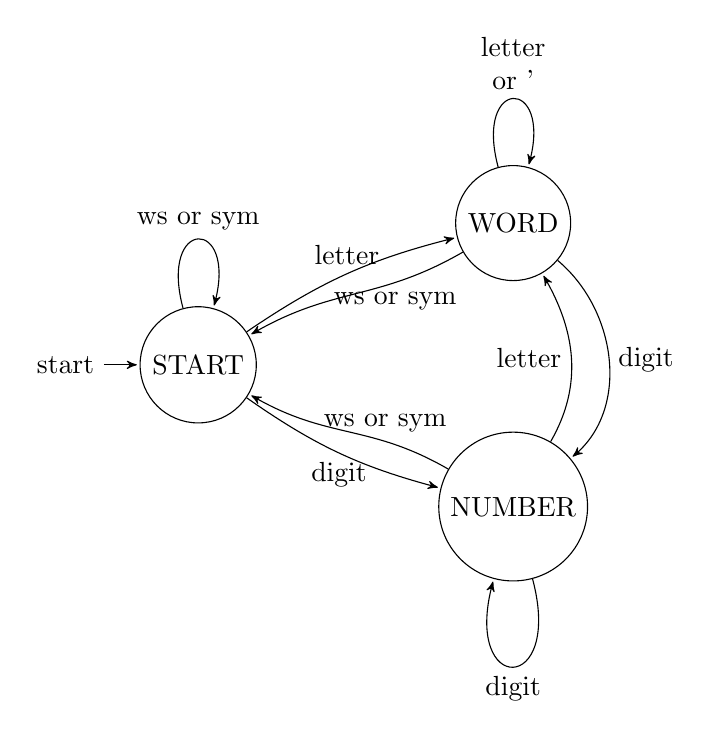
\begin{tikzpicture}[
        >=stealth',
        shorten >=1pt,
        node distance=4cm,
        on grid,
        auto,
        state/.style={circle, draw, minimum size=1.4cm}
    ]

        % States
        \node[state, initial] (S) {START};
        \node[state, right=of S, yshift=1.8cm] (W) {WORD};
        \node[state, right=of S, yshift=-1.8cm] (N) {NUMBER};

        % START self-loops
        \path[->]
            (S) edge[loop above] node {ws or sym} ();
            % (S) edge[loop left]  node {sym} ();

        % From START to WORD / NUMBER
        \path[->]
            (S) edge[bend left=10]  node[above] {letter} (W)
            (S) edge[bend right=10] node[below] {digit} (N);

        % WORD state
        \path[->]
            (W) edge[loop above] node[align=center]{letter\\or '} ()
            (W) edge[out=210,in=30,looseness=1.1]
                    node[pos=0.3,below,align=center]{ws or sym} (S)
            (W) edge[out=-40,in=40,looseness=1.0]
                    node[right] {digit} (N);

        % NUMBER state
        \path[->]
            (N) edge[loop below] node {digit} ()
            (N) edge[out=150,in=-30,looseness=1.1]
                    node[pos=0.3,above,align=center]{ws or sym} (S)
            (N) edge[out=60,in=-60,looseness=1.0]
                    node[left] {letter} (W);

    \end{tikzpicture}
    \caption{DFA for DFA-based tokenizer (\texttt{DFATokenizer}).}
\end{figure}

This DFA can be formally described by the 5-tuple $(Q,\Sigma,\delta,q_0,F)$, where:
\begin{itemize}
    \item $Q = \{\text{START}, \text{WORD}, \text{NUMBER}\}$.
    \item $\Sigma$ is the set of all ASCII characters.
    \item $q_0 = \text{START}$.
    \item $F$ can be considered $\{\text{WORD}, \text{NUMBER}, \text{START}\}$, since after finishing the input we may be in any of these states; tokens are emitted based on the state before termination.
\end{itemize}

\subsection{Integration into the Program}

The \texttt{DFATokenizer} is implemented as a Python class with:
\begin{itemize}
    \item A member \texttt{state} storing the current DFA state.
    \item A buffer \texttt{current} storing the characters of the token being built.
    \item A list \texttt{tokens} storing the final tokens of type \texttt{WORD}, \texttt{NUMBER}, or \texttt{SYMBOL}.
\end{itemize}

After tokenization, word tokens are normalized to lowercase for convenience when comparing or printing. The resulting sequence of tokens represents a regular-language-level processing of the input string.

\section{Parsing and CFG Interpretation}

\subsection{Dependency Trees as Parse Trees}

For parsing, we use spaCy to obtain part-of-speech (POS) tags and dependency relations between tokens. For each input sentence, spaCy returns a set of tokens with:
\begin{itemize}
    \item \texttt{text}: the original token string.
    \item \texttt{pos\_}: the coarse POS tag (e.g., VERB, NOUN, AUX).
    \item \texttt{dep\_}: the dependency relation (e.g., ROOT, nsubj, dobj).
    \item \texttt{head}: the head of the dependency arc.
\end{itemize}

We construct our own parse tree structure using the \texttt{DepNode} data class:
\begin{verbatim}
@dataclass
class DepNode:
    text: str
    lemma: str
    pos: str
    dep: str
    children: List["DepNode"] = field(default_factory=list)
\end{verbatim}

The function \texttt{build\_dep\_tree(doc)} creates one \texttt{DepNode} per token and links them according to the dependency arcs. The token whose \texttt{head} is itself becomes the root of the tree (corresponding to the syntactic ROOT of the sentence).

\subsection{Relation to Context-Free Grammars}

A dependency tree can be related to a CFG-style phrase structure tree as follows:
\begin{itemize}
    \item The ROOT verb corresponds roughly to the head of the VP in a rule like $S \to NP\;VP$.
    \item A token with dependency label \texttt{nsubj} (nominal subject) corresponds to the NP on the left side of the sentence.
    \item Objects or complements correspond to NPs or PPs attached to the verb.
\end{itemize}

Instead of explicitly writing a CFG and running a parser, we use the dependency tree as a compact representation of a derivation in some underlying CFG. spaCy's model has implicitly learned such a grammar from data. Our code then reuses the resulting tree to check simple CFG-like constraints.

\subsection{Natural Sentence Heuristic}

We implement the following heuristic in the function \texttt{is\_likely\_natural\_sentence(doc)}:
\begin{enumerate}
    \item There is exactly one ROOT token in the dependency parse.
    \item The ROOT token has POS tag VERB or AUX (verb or auxiliary).
    \item There exists at least one token with dependency label \texttt{nsubj}, \texttt{nsubjpass}, or \texttt{csubj} (some form of subject).
\end{enumerate}

Intuitively, this corresponds to requiring the existence of a subject and a finite verb, as in the CFG rule
\[
S \to NP\;VP
\]
where $VP$ contains a verbal head. If these constraints are violated, the string is unlikely to be a well-formed declarative sentence in English.

\section{System Design and Implementation}

\subsection{Overall Architecture}

The complete pipeline in \texttt{main()} performs the following steps for each input sentence:
\begin{enumerate}
    \item Print the raw sentence.
    \item Run DFA-based tokenization using \texttt{DFATokenizer}.
    \item Run spaCy's pipeline to obtain tokens with POS and dependency labels.
    \item Build a custom dependency tree using \texttt{build\_dep\_tree}.
    \item Print a pretty-printed version of the dependency tree.
    \item Apply \texttt{is\_likely\_natural\_sentence} to decide if the sentence is likely natural.
\end{enumerate}

\subsection{Key Data Structures}

\begin{itemize}
    \item \texttt{Tok}: a data class representing a token with fields \texttt{type} and \texttt{value}. Types are \texttt{"WORD"}, \texttt{"NUMBER"}, and \texttt{"SYMBOL"}.
    \item \texttt{DFATokenizer}: encapsulates the DFA states, transition logic, and token emission.
    \item \texttt{DepNode}: represents a node of the parse tree with text, lemma, POS tag, dependency label, and children.
\end{itemize}

\subsection{Python Implementation}

\begin{lstlisting}[caption={Python implementation of DFA-based tokenizer and dependency-tree parser},label={lst:implementation}]
from dataclasses import dataclass, field
from typing import List, Optional
import spacy

@dataclass
class Tok:
    type: str   # "WORD", "NUMBER", "SYMBOL"
    value: str

class DFATokenizer:
    def __init__(self):
        self.state = "START"
        self.current = ""
        self.tokens: List[Tok] = []

    def reset(self):
        self.state = "START"
               self.current = ""
        self.tokens.clear()

    def emit(self, type_):
        if self.current:
            self.tokens.append(Tok(type_, self.current))
            self.current = ""

    def tokenize(self, text: str) -> List[Tok]:
        self.reset()
        for ch in text:
            if self.state == "START":
                if ch.isspace():
                    continue
                elif ch.isalpha():
                    self.state = "WORD"
                    self.current += ch
                elif ch.isdigit():
                    self.state = "NUMBER"
                    self.current += ch
                else:
                    self.tokens.append(Tok("SYMBOL", ch))

            elif self.state == "WORD":
                if ch.isalpha() or ch == "'":
                    self.current += ch
                else:
                    self.emit("WORD")
                    self.state = "START"
                    # reprocess ch
                    if ch.isspace():
                        continue
                    elif ch.isdigit():
                        self.state = "NUMBER"
                        self.current += ch
                    else:
                        self.tokens.append(Tok("SYMBOL", ch))

            elif self.state == "NUMBER":
                if ch.isdigit():
                    self.current += ch
                else:
                    self.emit("NUMBER")
                    self.state = "START"
                    # reprocess ch
                    if ch.isspace():
                        continue
                    elif ch.isalpha():
                        self.state = "WORD"
                        self.current += ch
                    else:
                        self.tokens.append(Tok("SYMBOL", ch))

        if self.state == "WORD":
            self.emit("WORD")
        elif self.state == "NUMBER":
            self.emit("NUMBER")

        # normalize words to lowercase for convenience
        norm = []
        for t in self.tokens:
            if t.type == "WORD":
                norm.append(Tok("WORD", t.value.lower()))
            else:
                norm.append(t)
        return norm

@dataclass
class DepNode:
    text: str
    lemma: str
    pos: str
    dep: str
    children: List["DepNode"] = field(default_factory=list)

    def pretty(self, level=0) -> str:
        indent = "  " * level
        out = f"{indent}{self.text} ({self.pos}, {self.dep})\n"
        for child in self.children:
            out += child.pretty(level + 1)
        return out


def build_dep_tree(doc) -> Optional[DepNode]:
    if len(doc) == 0:
        return None

    # Create nodes for each token
    nodes = [DepNode(t.text, t.lemma_, t.pos_, t.dep_) for t in doc]

    root = None
    for i, tok in enumerate(doc):
        if tok.head.i == tok.i:
            # This is the ROOT token
            root = nodes[i]
        else:
            head_node = nodes[tok.head.i]
            head_node.children.append(nodes[i])

    return root

def is_likely_natural_sentence(doc) -> bool:
    #exactly one ROOT, ROOT is a verb or auxiliar, at least one nominal subject
 #uusing spacy learned grammar as a reference, not defining our cfg 

    roots = [t for t in doc if t.dep_ == "ROOT"]
    if len(roots) != 1:
        return False

    root = roots[0]
    if root.pos_ not in ("VERB", "AUX"):
        return False

    has_subject = any(t.dep_ in ("nsubj", "nsubjpass", "csubj") for t in doc)
    if not has_subject:
        return False

    return True


def main():
    # load spacy model (predefined "grammar")
    # make sure you installed it first:
    #   python -m spacy download en_core_web_sm
    nlp = spacy.load("en_core_web_sm")

    sentences = [
        "The man saw a dog.",
        "cat table green quickly.",
        "I will build a parser using automata.",
        "x1 + x2 = 10"
    ]

    tokenizer = DFATokenizer()

    for s in sentences:
        print("=" * 60)
        print("Sentence:", s)

        #  low-level DFA tokenization
        my_tokens = tokenizer.tokenize(s)
        print("\nDFA tokens:")
        for t in my_tokens:
            print(" ", t)

        # spacy analysis
        doc = nlp(s)

        print("\nspaCy tokens / POS / dep (reference grammar):")
        for t in doc:
            print(f"  {t.i:2d}: {t.text:10s} POS={t.pos_:6s} DEP={t.dep_:10s} HEAD={t.head.i}")

        # Use spacy arcs to build our parse tree
        tree = build_dep_tree(doc)
        print("\nOur dependency tree (built manually):")
        if tree:
            print(tree.pretty().rstrip())
        else:
            print("  <empty>")

        print("\nLikely natural language sentence?",
              "YES" if is_likely_natural_sentence(doc) else "NO")


if __name__ == "__main__":
    main()
\end{lstlisting}
\subsection{Source Code Repository}

The complete source code for this project is available on GitHub at:
\url{https://github.com/Karvy-Singh/TOCSuper.git}
\subsection{Example Sentences}

We tested the system on four sentences:
\begin{enumerate}
    \item \texttt{``The man saw a dog.''}
    \item \texttt{``cat table green quickly.''}
    \item \texttt{``I will build a parser using automata.''}
    \item \texttt{``x1 + x2 = 10''}
\end{enumerate}

For each sentence, the program prints:
\begin{itemize}
    \item The DFA tokens (type and value).
    \item spaCy tokens with POS and dependency labels.
    \item The custom dependency tree.
    \item The result of the natural sentence heuristic.
\end{itemize}

\section{Program Output}

\begin{figure}[H]
    \centering
    \includegraphics[width=0.6\textwidth]{output_sentence1}
    \caption{Program output for the sentence ``The man saw a dog.''}
    \label{fig:out1}
\end{figure}

\begin{figure}[H]
    \centering
    \includegraphics[width=0.6\textwidth]{output_sentence2}
    \caption{Program output for the sentence ``cat table green quickly.''}
    \label{fig:out2}
\end{figure}

\begin{figure}[H]
    \centering
    \includegraphics[width=0.6\textwidth]{output_sentence3}
    \caption{Program output for the sentence ``I will build a parser using automata.''}
    \label{fig:out3}
\end{figure}

\begin{figure}[H]
    \centering
    \includegraphics[width=0.6\textwidth]{output_sentence4}
    \caption{Program output for the expression ``x1 + x2 = 10''.}
    \label{fig:out4}
\end{figure}

\section{Results and Discussion}

\subsection{Tokenization Behavior}

For the sentence \texttt{``The man saw a dog.''}, the DFA produces tokens similar to:
\begin{center}
\begin{tabular}{ll}
\toprule
Type & Value \\
\midrule
WORD   & the \\
WORD   & man \\
WORD   & saw \\
WORD   & a \\
WORD   & dog \\
SYMBOL & . \\
\bottomrule
\end{tabular}
\end{center}

This shows that the tokenizer correctly distinguishes word tokens and punctuation symbols. Numbers or mathematical expressions such as \texttt{``x1 + x2 = 10''} generate a mix of \texttt{WORD}, \texttt{NUMBER}, and \texttt{SYMBOL} tokens, demonstrating how DFA-based tokenization can be used for both natural language and simple formulas.

\subsection{Natural Sentence Classification}

Table~\ref{tab:results} summarizes the heuristic classification results for the four example sentences.

\begin{table}[H]
	\centering
	\caption{Heuristic judgment of whether a sentence is likely natural.}
	\label{tab:results}
	\begin{tabular}{p{7cm}c}
		\toprule
		Sentence & Likely Natural? \\
		\midrule
		The man saw a dog. & YES \\
		cat table green quickly. & NO \\
		I will build a parser using automata. & YES \\
		x1 + x2 = 10 & NO \\
		\bottomrule
	\end{tabular}
\end{table}

The sentences that have a clear subject and verb (\texttt{``The man saw a dog.''} and \texttt{``I will build a parser using automata.''}) satisfy the heuristic. The purely nominal and adverbial sequence \texttt{``cat table green quickly.''} and the mathematical expression lack a proper verbal ROOT with a subject, so they are correctly classified as unlikely to be natural sentences.

\subsection{Connection to Automata and Grammars}

The project demonstrates the following connections:
\begin{itemize}
    \item The DFA tokenizer is a direct application of regular languages and deterministic finite automata studied in Theory of Computation.
    \item The dependency tree and the natural sentence heuristic are inspired by CFG ideas, where a valid sentence must expand from a start symbol $S$ to valid constituents like NP and VP.
    \item By combining a DFA-based front-end with a CFG-style parsing back-end (implemented using spaCy's learned grammar), we obtain a practical yet theoretically grounded NLP pipeline.
\end{itemize}

\section{Conclusion and Future Work}

In this project, we implemented a small natural language processing system that combines:
\begin{itemize}
    \item A deterministic finite automaton for tokenizing input strings into words, numbers, and symbols.
    \item A dependency-tree-based representation of sentence structure derived from spaCy.
    \item A simple context-free-grammar-inspired heuristic for detecting whether a sentence is likely to be a natural English sentence.
\end{itemize}

This work illustrates how abstract theoretical models such as DFA and CFG can be embedded into concrete applications. Even though modern NLP heavily uses statistical and neural methods, the underlying notions of tokens, parse trees, and grammatical constraints remain rooted in the theory of computation.

Possible directions for future work include:
\begin{itemize}
    \item Designing an explicit CFG for a subset of English and implementing a top-down or bottom-up parser to compare with the dependency-based approach.
    \item Extending the DFA tokenizer to handle more complex token types, such as multi-word tokens or abbreviations.
    \item Incorporating additional grammatical features (e.g., object presence, agreement, tense) into the natural sentence heuristic.
    \item Evaluating the system on a larger set of sentences and analyzing false positives and false negatives.
\end{itemize}

\section*{References}

\begin{enumerate}
    \item Hopcroft, J.E., Motwani, R., Ullman, J.D. \textit{Introduction to Automata Theory, Languages, and Computation}. Pearson.
    \item Sipser, M. \textit{Introduction to the Theory of Computation}. Cengage Learning.
    \item Jurafsky, D., Martin, J.H. \textit{Speech and Language Processing}. Pearson.
    \item spaCy Documentation: \url{https://spacy.io/}
    \item NLTK Documentation: \url{https://www.nltk.org/howto/parse.html}
\end{enumerate}

\end{document}
